%%%%%%%%%%%%%%%%%%%%%%%%%%%%%%%%%%%%%%%%%
% a0poster Portrait Poster
% LaTeX Template
% Version 1.0 (22/06/13)
%
% The a0poster class was created by:
% Gerlinde Kettl and Matthias Weiser (tex@kettl.de)
% 
% This template has been downloaded from:
% http://www.LaTeXTemplates.com
%
% License:
% CC BY-NC-SA 3.0 (http://creativecommons.org/licenses/by-nc-sa/3.0/)
%
%%%%%%%%%%%%%%%%%%%%%%%%%%%%%%%%%%%%%%%%%

%----------------------------------------------------------------------------------------
%	PACKAGES AND OTHER DOCUMENT CONFIGURATIONS
%----------------------------------------------------------------------------------------

\documentclass[a0,portrait]{a0poster}

\usepackage[utf8]{inputenc} %para aceitar carcteres da língua portuguesa
\usepackage[brazil]{babel}
\setlength\parindent{30pt}

\usepackage{multicol} % This is so we can have multiple columns of text side-by-side
\columnsep=100pt % This is the amount of white space between the columns in the poster
\columnseprule=3pt % This is the thickness of the black line between the columns in the poster

\usepackage[svgnames]{xcolor} % Specify colors by their 'svgnames', for a full list of all colors available see here: http://www.latextemplates.com/svgnames-colors

\usepackage{times} % Use the times font
%\usepackage{palatino} % Uncomment to use the Palatino font

\usepackage{graphicx, float} % Required for including images
%\graphicspath{{figures/}} % Location of the graphics files
\usepackage{booktabs} % Top and bottom rules for table
\usepackage[font=small,labelfont=bf]{caption} % Required for specifying captions to tables and figures
\usepackage{amsfonts, amsmath, amsthm, amssymb, cases} % For math fonts, symbols and environments
%\usepackage{wrapfig} % Allows wrapping text around tables and figures

\begin{document}

%----------------------------------------------------------------------------------------
%	POSTER HEADER 
%----------------------------------------------------------------------------------------

% The header is divided into two boxes:
% The first is 75% wide and houses the title, subtitle, names, university/organization and contact information
% The second is 25% wide and houses a logo for your university/organization or a photo of you
% The widths of these boxes can be easily edited to accommodate your content as you see fit

\begin{minipage}[b]{0.12\linewidth}

\includegraphics[width=12cm]{imgs/fap.jpg} \vspace{1cm}\\
\thinspace 
\includegraphics[width=8cm]{imgs/laralogo2.png}\\
\end{minipage}
%
\begin{minipage}[b]{0.75\linewidth}
{\centering
%\veryHuge \color{NavyBlue} \textbf{Projeto e Controle  de Processo com Controle de Nível, Vazão e Temperatura} \color{Black}\\[2cm] % Title
\fontsize{80}{120} \color{NavyBlue} \textbf{Controle Fuzzy de Bancada Industrial} \color{Black}\\[1.5cm] % Title

%\Huge\textit{An Exploration of Complexity}\\[2cm] % Subtitle
\huge \textsc{Jhonantans M. Rocha e Eduardo S. Tognetti}\\[0.5cm] % Author(s)

\Large{\bf Departamento de Engenharia Elétrica, ENE/FT/UnB, Brasília, DF, Brasil}\\[0.5cm]
\Large{\bf Semana Universitária 2016: }
\large{\bf Diferenças que somam, ideias que multiplicam}\\[0.5cm]
\Large Emails: \texttt{jhmrocha@gmail.com e estognetti@ene.unb.br}\\
}
\end{minipage}
%
\begin{minipage}[b]{0.12\linewidth}

\includegraphics[width=8cm]{imgs/logo.png} \vspace{3cm}\\

\includegraphics[width=8cm]{imgs/cnpq.jpg}\\
\end{minipage}

\vspace{2cm} % A bit of extra whitespace between the header and poster content

%----------------------------------------------------------------------------------------

\begin{multicols}{2} % This is how many columns your poster will be broken into, a portrait poster is generally split into 2 columns

%----------------------------------------------------------------------------------------
%	RESUMO
%----------------------------------------------------------------------------------------

\color{NavyBlue} % Navy color for the abstract
\begin{abstract}

\fontsize{18}{22}
Trata-se neste projeto da aplicação da modelagem fuzzy para um sistema industrial multivariável. Busca-se aqui uma forma mais efetiva de aliar a linearização de sistemas mantendo o comportamento o mais próximo possível do original.


\end{abstract}
\vspace{0.5cm}
%----------------------------------------------------------------------------------------
%	INTRODUÇÃO
%----------------------------------------------------------------------------------------
%\fontsize{45}{55}

\color{DarkSlateGray} % SaddleBrown color for the introduction

\section*{Introdução}

\color{Black}

Desenvolver controladores para sistemas não-lineares é quase sempre uma tarefa dispendiosa e complexa devido à dificuldade em aplicar as táticas convencionais de controle a estes problemas. Para plantas industriais multivariáveis essa complexidade é ainda maior, já que os graus de acoplamento entre as variáveis presentes já apresentam um desafio na sintonia do controlador.  
%----------------------------------------------------------------------------------------
%	DESCRIÇÃO DO SISTEMA
%----------------------------------------------------------------------------------------
\vspace{1cm}
\color{DarkSlateGray} % DarkSlateGray color for the rest of the content

\section*{Descrição do Sistema}

\color{Black}

Este trabalho apresenta a utilização da modelagem fuzzy de uma planta de quatro tanques proposta por Johansson, como na figura a seguir:

\indent A figura a seguir apresenta um esquemático do projeto:

\begin{center}\vspace{1.5cm}
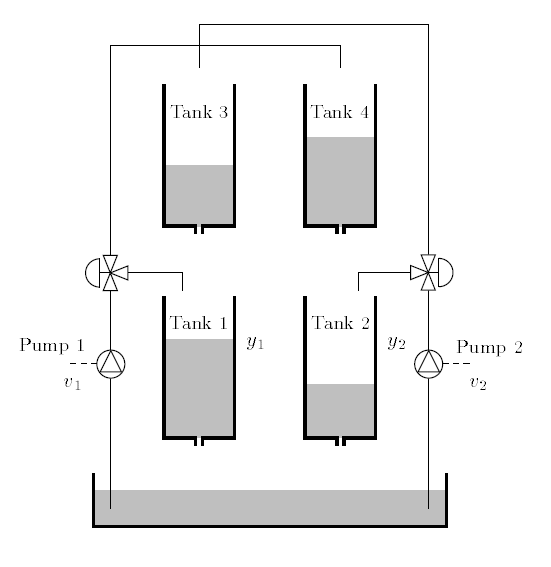
\includegraphics[width=0.5\linewidth]{imgs/4tank.png}
\captionof{figure}{Sistema de Quatro-Tanques.}
\end{center}
\vspace{1.5cm}

%----------------------------------------------------------------------------------------
%	MODELAGEM MATEMÁTICA
%----------------------------------------------------------------------------------------
\vspace{1cm}
\color{DarkSlateGray} % SaddleBrown color for the introduction

\subsection*{Modelagem Matemática}

\color{Black}

As equações não lineares que descrevem este sistema são dadas por:

\vspace{0.2cm}
\begin{equation}
	\begin{cases}
		\dot{h_{1}} = \frac{1}{A_{1}}(o_{3}\sqrt{2gh_{3}} + \gamma_{1}k_{1}v_{1} - o_{1}\sqrt{2gh_{1}})\\
		
		\dot{h_{2}} = \frac{1}{A_{2}}(o_{4}\sqrt{2gh_{4}} + \gamma_{2}k_{2}v_{2} - o_{2}\sqrt{2gh_{2}})\\
		
		\dot{h_{3}} = \frac{1}{A_{3}}((1 - \gamma_{2})k_{2}v_{2} - o_{3}\sqrt{2gh_{3}})\\
		
		\dot{h_{4}} = \frac{1}{A_{4}}((1 - \gamma_{1})k_{1}v_{1} - o_{4}\sqrt{2gh_{4}})
	\end{cases}
\end{equation}
\vspace{0.4cm}

É prática comum recorrer-se à linearização, geralmente por série de Taylor, das equações desses sistemas. Desta forma, consegue-se uma aproximação do sistema inicial, idealizada a partir de um ponto de referência, sem funções não lineares em sua representação:

\vspace{0.2cm}
\begin{equation}
	\dot{h}(t) =  Ah(t) + Bu(t)
\end{equation}
\vspace{0.4cm}


O sistema resultante deste simples processo é exato no ponto de linearização, porém à medida que as variáveis controladas e manipuladas se afastam do ponto de operação, o ponto de referência da linearização, o modelo passa a se afastar da planta real.

\begin{figure}[H]
	\centering
	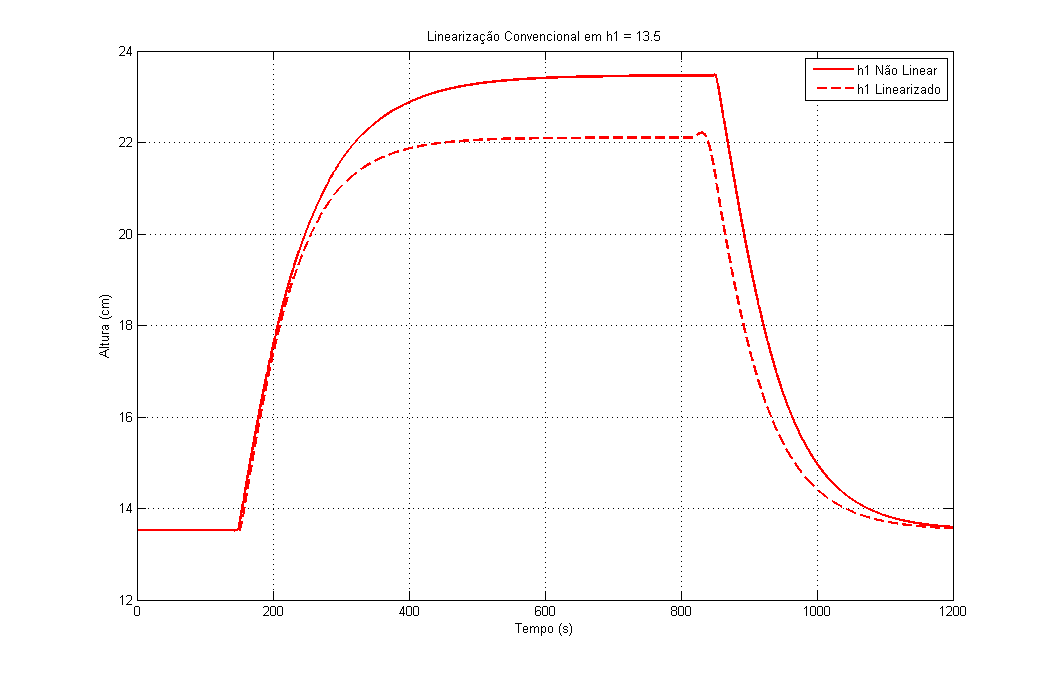
\includegraphics[width=0.4\textwidth]{imgs/v2_linear_conv.png}
	\caption{Linearização convencional}
	\label{figLinConv}
\end{figure}

%----------------------------------------------------------------------------------------
%	SISTEMAS FUZZY
%----------------------------------------------------------------------------------------

\vspace{1cm}
\color{DarkSlateGray} % SaddleBrown color for the introduction

\section*{Modelagem Fuzzy}

\color{Black}

A utilização da metodologia fuzzy oferece formas de aproveitar as vantagens da linearização e amenizar suas discrepâncias em relação ao modelo real. O modelo proposto por Takagi e Sugeno consiste na linearização do sistema em mais de um ponto de operação, obtendo assim vários modelos lineares. 

Estes pontos são escolhidos como para expressar, em variáveis linguísticas, os estados desejados do sistema. No caso de um sistema de quatro-tanques, poderíamos utilizar, para cada nível controlado, o conjunto {nível baixo, nível alto}. Para um conjunto de dois tanques controlados obtém-se quatro sistemas lineares:

\begin{center}
	\begin{minipage}{.2\textwidth}
		\begin{itemize}
			\item Se h1 é baixo e h2 é baixo, então: \\
			$(h(t)) = A_1h(t)+B_1u(t)$
			\item Se h1 é baixo e h2 é alto, então: \\
			$(h(t)) = A_2h(t)+B_2u(t)$
			\item Se h1 é alto e h2 é baixo, então: \\
			$(h(t)) = A_3h(t)+B_3u(t)$
			\item Se h1 é alto e h2 é alto, então: \\
			$(h(t)) = A_4h(t)+B_4u(t)$
		\end{itemize}
	\end{minipage}
\end{center}

Faz-se então o cálculo e verifica-se o grau de pertinência de cada um dos dois níveis, em tempo real, à cada uma das zonas do conjunto linguístico. Nota-se que as função de pertinência assume valores no conjunto [0,1], sendo 0 quando o nível está completamente fora da zona que o define e 1 quando é exatamente o valor do ponto de operação. O modelo final é pela soma sistemas linearizados ponderada pelos índices de pertinência em cada uma delas:

\begin{equation}
	\dot{h} = \sum_{i=1}^{4} \dfrac{w_i(h)(A_ih+Bu)}{\sum_{j=1}^{4}w_i(h)}
\end{equation}

%----------------------------------------------------------------------------------------
%	RESULTADOS
%----------------------------------------------------------------------------------------
\vspace{1cm}
\color{DarkSlateGray} % SaddleBrown color for the introduction

\section*{Simulações e Resultados}

\color{Black}

As imagens a seguir apresentam os resultados para modelagens fuzzy com 2 ou mais níveis no conjunto de variáveis linguísticas.

\begin{figure}[H]
	\centering
	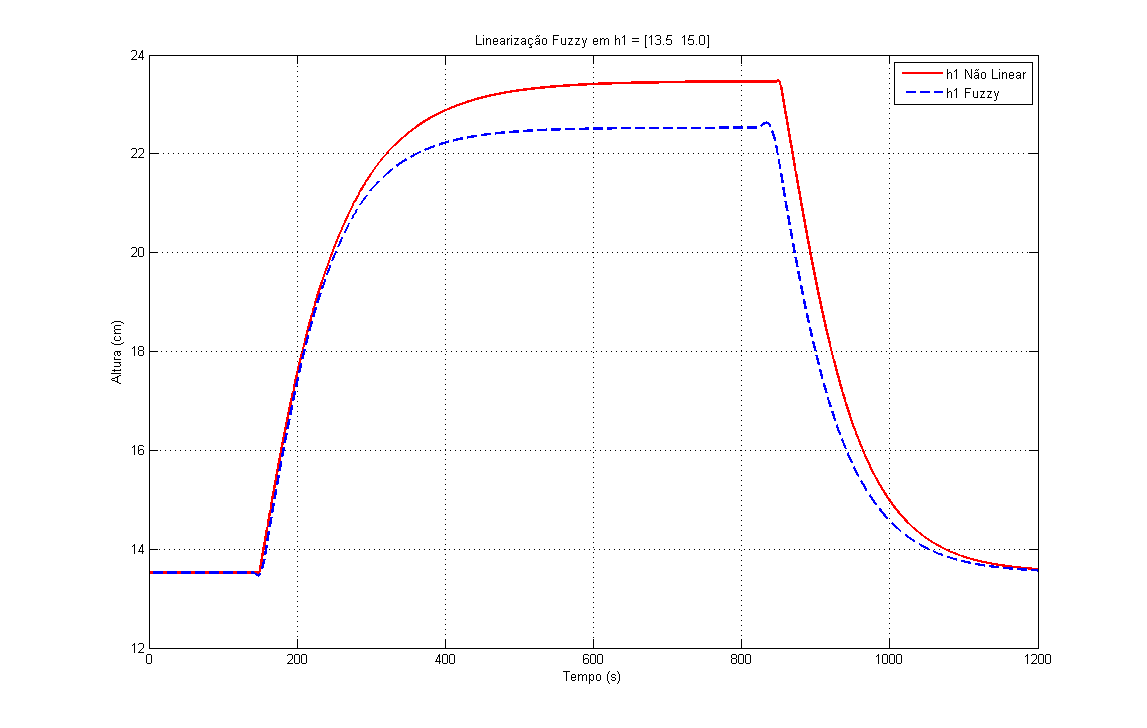
\includegraphics[width=0.4\textwidth]{imgs/v2_linear_fuzzy_13_15.png}
	\caption{Linearização Fuzzy em {13, 15}}
	\label{figFuzzy13_15}
\end{figure}

\begin{figure}[H]
	\centering
	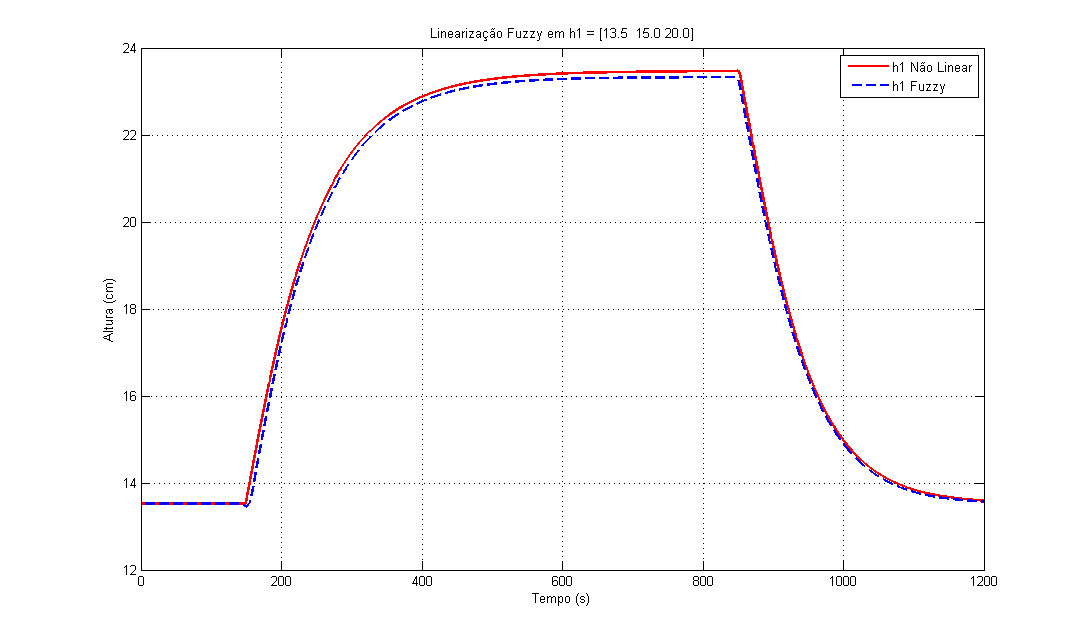
\includegraphics[width=0.4\textwidth]{imgs/v2_linear_fuzzy_13_15_20.png}
	\caption{Linearização Fuzzy em {13, 15, 20}}
	\label{figFuzzy13_15_20}
\end{figure}

%----------------------------------------------------------------------------------------
%	CONCLUSÃO
%----------------------------------------------------------------------------------------
\color{DarkSlateGray} % SaddleBrown color for the introduction

\section*{Conclusão}

\color{Black}

O objetivo final da modelagem fuzzy de um sistema não-linear é obter um conjunto finito de modelos lineares e simples que o definam bem em várias faixas de operação.  Mostrou-se neste trabalho a eficácia desta técnica para um sistema industrial multivariável. 

Futuros trabalhos incluem a aplicação de técnicas de controle clássico a partir dos modelos obtidos e seguir os mesmos procedimentos para formação da regra geral de controle. Por fim, a validação dos modelos obtidos em uma planta real e sua aplicação em controlador lógico programável.


%----------------------------------------------------------------------------------------

\end{multicols}
\end{document}
